\section{Zielsetzung}
\label{sec:Zielsetzung}
Das Ziel des Versuchs ist es, die Schwingungsdauer und Schwebungsdauer bei gekoppelten Pendeln in verschiedenen Schwingungsarten zu bestimmen.

\section{Theorie}
\label{sec:Theorie}

\subsection{Das Fadenpendel} % (fold)
\label{sub:Fadenpendel}
Das Fadenpendel besteht aus einer Masse $m$ und einem Faden der Länge $l$, wobei dieser idealerweise keine Masse besitzt.
Es wirkt die Gewichtskraft $F=m\,\vec{a}$ als rücktreibende Kraft bei der Auslenkung des Pendels aus seiner Ruhelage.
Dadurch entsteht ein Drehmoment $M=D_p\, \phi$ auf das Pendel, wobei $\phi$ der Auslenkwinkel und $D_p$ die Winkelrichtung des Pendels ist.
Für kleine Auslenkungen gilt die Kleinwinkelnäherung, sodass die Bewegungsgleichung
\begin{equation*}
    J \, \ddot{\phi} + D_p \, \phi = 0
\end{equation*}
lautet, mit $J$ als Trägheitsmoment.
Die Lösung der Gleichung beschreibt eine harmonische Schwingung mit der Schwingungsfrequenz
\begin{equation*}
    \omega = \sqrt{\frac{D_p}{J}} = \sqrt{\frac{g}{l}}.
\end{equation*}
Bei kleinen Auslenkungen ist die Schwingungsdauer somit unabhängig von den Pendelmassen und dem Auslenkungswinkel.
 
% subsection Fadenpendel (end)

\subsection{Kopplung zweier Pendel} % (fold)
\label{subsec:Schwingungen}
 Bei der Kopplung zweier identischer Pendel durch eine Feder wirkt ein weiteres Drehmoment auf jedes Pendel.
 Dadurch, dass die Pendel jetzt über eine Feder gekoppelt sind, schwingen sie nicht mehr unabhängig voneinander und es gilt das Hookesche Gesetz
 \begin{equation*}
     F(x) = -k \, x ,
 \end{equation*}
 wobei $k$ die Federkonstante und $x$ die Auslenkung ist.
 Die Bewegungsgleichung wird zu einem System gekoppelter Differentialgleichungen
 \begin{align*}
     J \, \ddot{\phi_1} + D \phi_1 &= D_F (\phi_2 - \phi_1) \\
     J \, \ddot{\phi_2} + D \phi_2 &= D_F (\phi_1 - \phi_2)
 \end{align*}
 umgeformt, wobei die linke Seite der Gleichungen die Schwingung des einzelnen Pendels ist und die rechte Seite die Kopplung der Pendel betrachtet.
 Die Schwingungsgleichungen können bei der richtigen Wahl der Winkel entkoppelt werden und so als eine Überlagerung zweier Eigenschwingungen betrachtet werden.
 Abhängig von den Anfangsbedingungen $\phi(0)$ und $\dot{\phi}(0)$ gibt es verschiedene Schwingungsarten, die im Folgenden näher beschrieben werden.

\subsubsection{Gleichsinnige Schwingungen}
\label{subsec:Gleich}
\begin{minipage}[t]{0.5\textwidth}
Bei einer gleichsinnigen Schwingung werden zwei identische Pendel um den gleichen Winkel $\phi_1 = \phi_2$ ausgelenkt, sodass die Kopplungsfeder keine Kraft auf die Pendel ausübt.
Die rücktreibende Kraft wird nur von der Gravitation verursacht.
Mit der Schwingungsfrequenz der gleichsinnigen Schwingung
\begin{equation}
    \omega_+ = \sqrt{\frac{g}{l}}
    \label{eqn:omega+}
\end{equation}
ergibt sich die Schwingungsdauer zu
\begin{equation}
    T_+ = 2 \pi \sqrt{\frac{l}{g}}.
    \label{eqn:T+}
\end{equation}
\end{minipage}
\begin{minipage}[t]{0.5\textwidth}
    \begin{figure}[H]
        \centering
        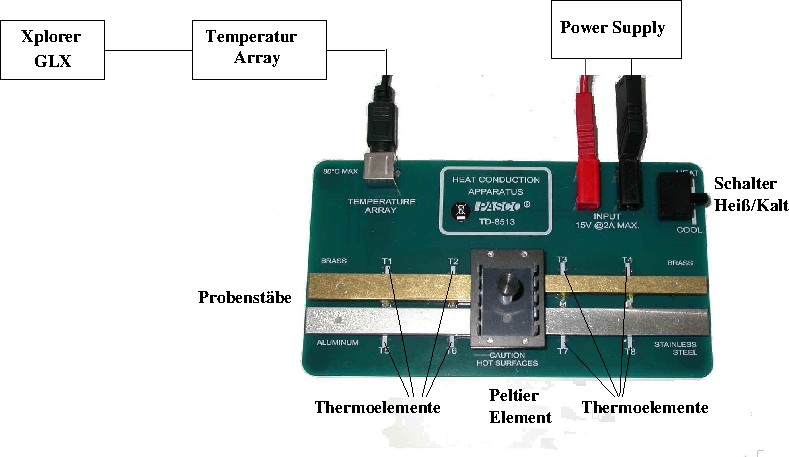
\includegraphics[width=0.45\textwidth]{build/Abb_1.pdf}
\caption{\\Abbild der gleichsinnigen Schwingung. \cite{V106}}
        \label{fig:gleich}
      \end{figure}
\end{minipage}
\subsubsection{Gegensinnige Schwingung}

\begin{minipage}[t]{0.5\textwidth}
\label{subsec:Gegen}
Im Gegensatz zur gleichsinnigen Schwingung werden bei der gegensinnigen Schwingung zwei identischen Pendel um den entgegengesetzten Winkel $\phi_1 = -\phi_2$ ausgelenkt.
In diesem Fall übt die Kopplungsfeder eine jeweils gleich große, aber entgegengesetzte Kraft auf die einzelnen Pendel aus.
Mit der Schwingungsfrequenz
\begin{equation}
    \omega_- = \sqrt{\frac{g}{l} + \frac{2K}{l}}
    \label{eqn:omega-}
\end{equation}
der symmetrischen Schwingung ergibt sich die Schwingungsdauer
\begin{equation}
    T_- = 2\pi \sqrt{\frac{l}{g+2K}},
    \label{eqn:T-}
\end{equation}
wobei die Kopplungskonstante der Feder durch $K$ dargestellt wird.
\end{minipage}
\begin{minipage}[t]{0.5\textwidth}
    \begin{figure}[H]
        \centering
        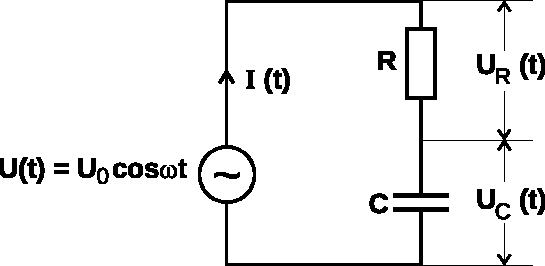
\includegraphics[width=0.5\textwidth]{build/Abb_2.pdf}
        \caption{Abbild der \\gegensinnigen Schwingung. \cite{V106}}
        \label{fig:gegen}
      \end{figure}
\end{minipage}
\subsubsection{Gekoppelte Schwingungen}
\label{subsec:Gekoppelt}
\begin{minipage}[t]{0.5\textwidth}
Im Fall der gekoppelten Schwingung bleibt eines der Pendel in Ruhelage $\phi_1=0$ und das andere identische Pendel wird um den Winkel $\phi_2 \neq 0$ ausgelenkt.
Beim Schwingen überträgt das erste Pendel seine Energie auf das Zweite, sodass das Zweite langsam anfängt zu schwingen und das Erste langsamer wird, bis es stillsteht.
Das zweite Pendel überträgt nun seine Energie wieder auf das Erste, welches anfängt zu schwingen.
Die Amplituden sind wie eine Glockenkurve. 
Ihr Maximum erreichen sie jeweils dann, wenn das andere Pendel zur Ruhe kommt.
Diese vollständige Energieübertragung wiederholt sich immer wieder und die Zeit zwischen zwei Stillständen eines Pendels wird Schwebungsdauer 
\begin{equation}
    T_S=\frac{T_+ + T_-}{T_+-T_-}
    \label{eqn:TS}
\end{equation}
genannt. Diese und die Schwebungsfrequenz
\begin{equation}
    \omega_S = \omega_+ - \omega_-
    \label{eqn:omegaS}
\end{equation}
werden durch die Schwingungsdauer der gleichsinnigen Schwingung $T_+$ und der gegensinnigen Schwingung $T_-$ bestimmt.

\end{minipage}
\begin{minipage}[t]{0.5\textwidth}
    \begin{figure}[H]
        \centering
        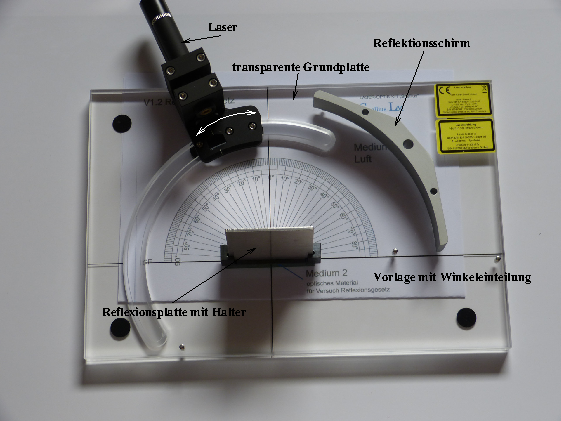
\includegraphics[width=0.6\textwidth]{build/Abb_3.pdf}
        \caption{Abbild der \\gekoppelten Schwingung. \cite{V106}}
        \label{fig:gekoppelt}
      \end{figure}
\end{minipage}

Die Kopplungskonstante
\begin{equation}
    K = \frac{\omega_-^2 -\omega_+^2}{\omega_-^2 + \omega_+^2} = \frac{T_+^2 - T_-^2}{T_+^2 + T_-^2}
    \label{eqn:K}
\end{equation}
der Feder wird als Maß für die Kopplung angesehen.
 % subsection Gekoppelte Schwingungen (end)